\begin{figure}[!htbp]
\begin{center}
\resizebox{0.5\textwidth}{!}{
\begin{tikzpicture}[
roundnode/.style={circle, draw=black!60, fill=green!60, very thick, minimum size=2mm},
]
%nodes
\node[inner sep=0pt] at (-10, 9){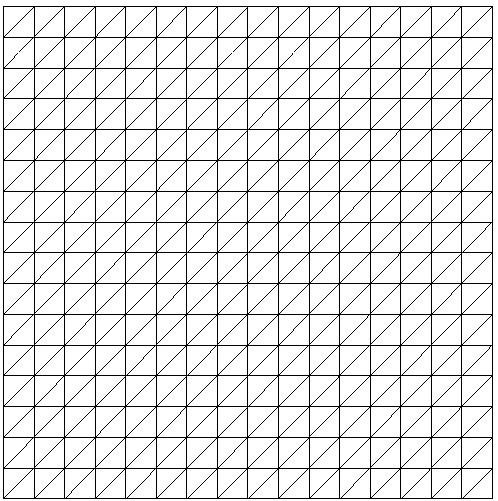
\includegraphics[width=0.15\textwidth]{figures/grid2.png}};
\node[roundnode] at (-3,9) (A){};
\node[above of=A]{\tiny \begin{tabular}{c}
  Input $x$\\\hline
  Initial Guess $u_0$\\ $r_0=f-A_1u_0$
\end{tabular}};
\node[roundnode] at (-4,9) (B){};
\node[left=1mm of B]{\tiny \begin{tabular}{c}
  $f^1 =F^1(x)$\\\hline
%$v_1=u_0+S_1r_0$\\
%$ r_1=f-A_1v_1$
$r_1 = F_1(r^0)$
\end{tabular} };
\node[inner sep=0pt] at (-10, 6){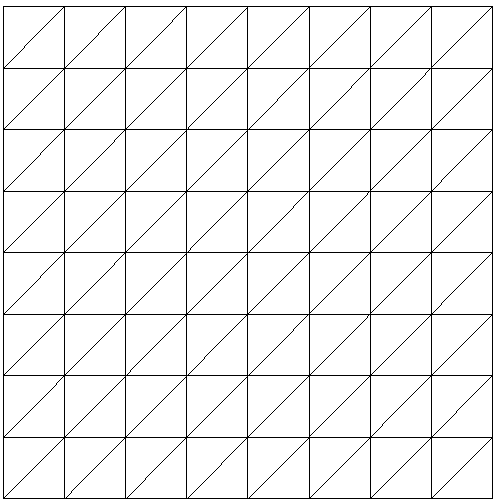
\includegraphics[width=0.15\textwidth]{figures/grid1.png}};
\node[roundnode] at (-3,6)  (C){};
\node[left=1mm of C]{\tiny \begin{tabular}{c}
$f^2=F^2(R_1^2f^1)$ \\\hline
%$v_2=S_2R_1^2r_1$\\ $r_2= R_1^2r_1-A_2v_2$
$r_2 = F_2(R^2_1r_1)$
\end{tabular} };
\node[inner sep=0pt] at (-10, 3){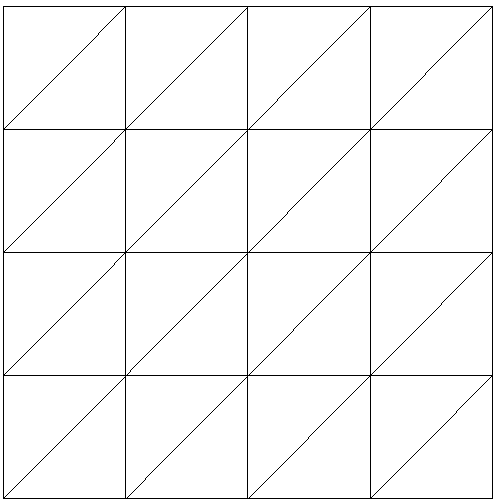
\includegraphics[width=0.15\textwidth]{figures/grid0.png}};
\node[roundnode] at (-2,3)  (D){};
\node[left=1mm of D]{\tiny \begin{tabular}{c}
$f^3=F^3(R_2^3f^2)$ \\\hline
%$v_3=S_3R_2^3r_2$\\ $r_3= R_2^3r_2-A_3v_3$
$r_3 = F_3(R^3_2r_2)$
\end{tabular} };
\node[inner sep=0pt] at (-10, 0){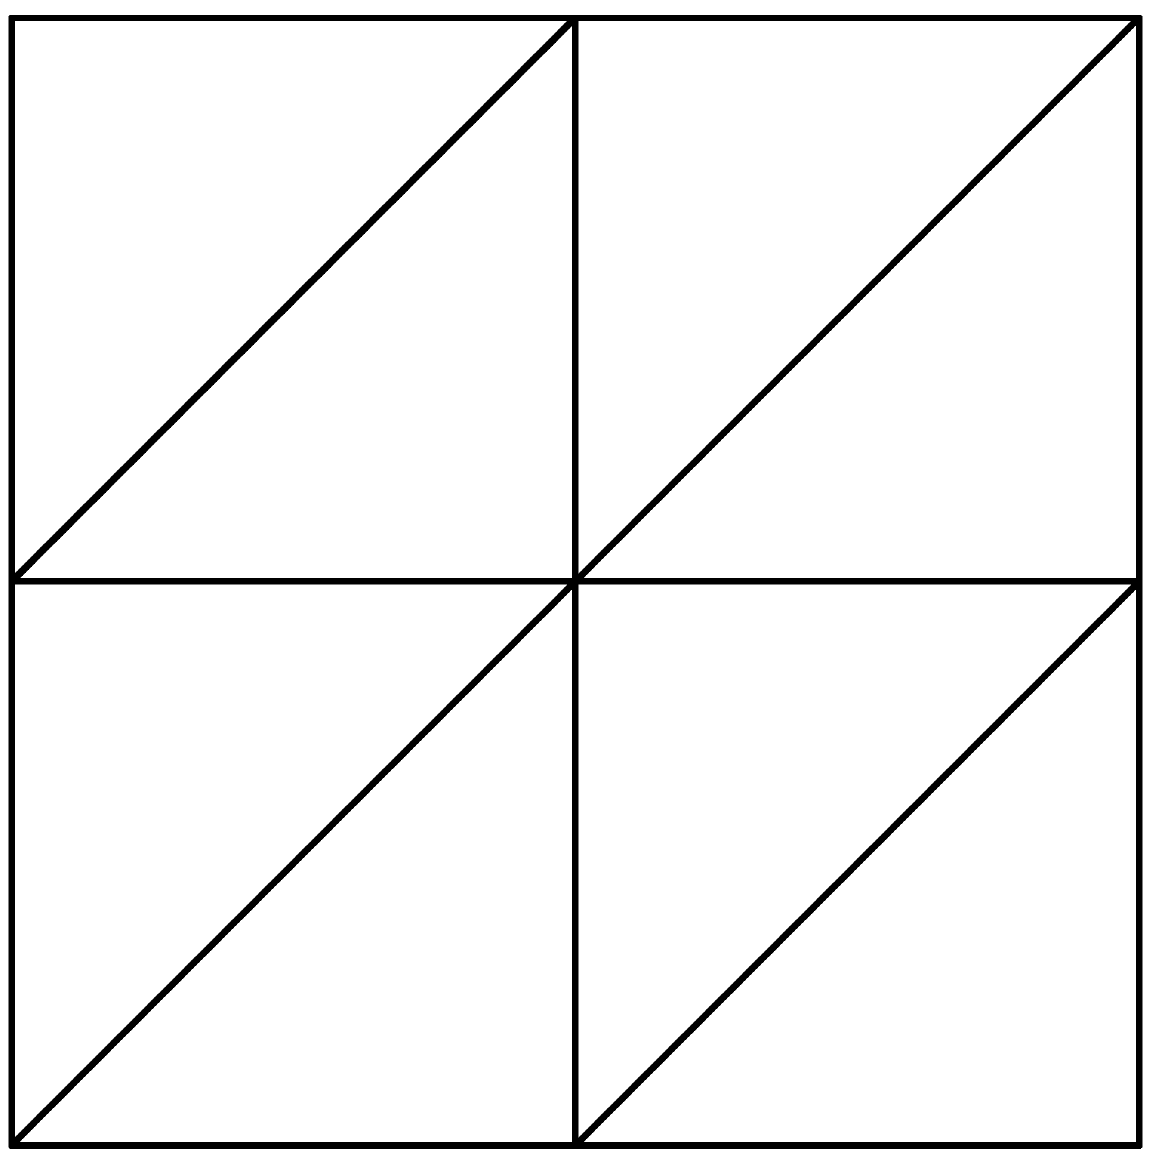
\includegraphics[width=0.15\textwidth]{figures/grid.png}};
\node[roundnode] at (-1,0)  (E){};
\node[below of=E]{\tiny \begin{tabular}{c}
$g^4=f^4=F^4(R_3^4f^3)$ \\\hline
$v_4= r_4 = F_4(R_3^4r_3)$
\end{tabular} };
\node[roundnode] at (0,3)  (F){};
\node[right=1mm of F]{\tiny \begin{tabular}{c}
$g^3 = G^3(P_4^3g^4)$  \\\hline
%$v_3\leftarrow v_3+(R_3^4)^Tv_4$ \\ $r_3=S_3(R_2^3r_2-A_3v_3)$\\ $v_3\leftarrow v_3+r_3$
$v_3 = G_3(P^3_4v_4)$
\end{tabular} };
\node[roundnode] at (1,6)  (G){};
\node[right=1mm of G]{\tiny \begin{tabular}{c}
$g^2 = G^2(P_3^2g^3)$  \\\hline
%$v_2\leftarrow v_2+(R_2^3)^Tv_3$ \\ $r_2=S_2(R_1^2r_1-A_2v_2)$\\ $v_2\leftarrow v_2+r_2$
$v_2 = G_2(P^2_3v_3)$
\end{tabular} };
\node[roundnode] at (2,9)  (H){};
\node[right=1mm of H]{\tiny \begin{tabular}{c}
$g^1 = G^1(P_2^1g^2)$  \\\hline
%$v_1\leftarrow v_1+(R_1^2)^Tv_2$ \\ $r_1=S_1(f-A_1v_1)$\\ $v_1\leftarrow v_1+r_1$
$v_1 = G_2(P^1_2v_2)$
\end{tabular} };
\node[roundnode] at (1,9)  (I){};
\node[above of=I]{\tiny \begin{tabular}{c}
  Output $y=ResNet(x)$\\\hline
  Solution $u\leftarrow u_0+B_\vee r_0$
\end{tabular}};
% lines
\draw[ultra thick, ->] (A)--(B) node[pos=.5,above,sloped] (TextNode) {};
\draw[ultra thick, ->] (B)--(C) node[pos=.5,above,sloped] (TextNode){};
\draw[ultra thick, ->] (C)--(D) node[pos=.5,above,sloped] (TextNode){};
\draw[ultra thick, ->] (D)--(E) node[pos=.5,above,sloped] (TextNode){};
\draw[ultra thick, ->] (E)--(F) node[pos=.5,above,sloped] (TextNode){};
\draw[ultra thick, ->] (F)--(G) node[pos=.5,above,sloped] (TextNode){};
\draw[ultra thick, ->] (G)--(H) node[pos=.5,above,sloped] (TextNode){};
\draw[ultra thick, ->] (H)--(I) node[pos=.5,above,sloped] (TextNode){};
\end{tikzpicture} }
\caption{Left: a nested multilevel grids; Right: a ${\rm V}$-cycle multigrid method 
	%(see \eqref{multi-backslash}-\eqref{eq:slash}) 
	versus a CNN model for segmentation 
  %(see  \eqref{multi-encode}-\eqref{multi-decode}) 
  .}
\label{fig:V-cycle}
\end{center}
\end{figure}
